\section{ActiveClean}
This section describes an extension to SampleClean which includes Machine Learning.

\subsection{Motivation}
The growing popularity of predictive models in data analytics \cite{bdas, alexandrov2014stratosphere, crotty2014tupleware, hellerstein2012madlib} leads to additional challenges in managing dirty data.
Predictive models rely on learning relationships between features and labels, and systematic corruption \cite{taylor1982introduction} (i.e., corruption that disproportionately affects certain data) can mask or even introduce spurious new relationships.
Furthermore, the high dimensionality of these models can amplify small problems \cite{xiaofeature} resulting in error-prone predictions even when trained on mostly clean data.

Consider a music recommender system in which due to a software bug, all users from Europe have an incorrect age attribute defaulted to ``18-24".
A recommendation model trained on this data may spuriously learn a correlation relationship between age ``18-24" and music liked by European users.
A bug, which ostensibly affected only the European users' records, can affect predictions to all users aged ``18-24".
Systematic corruption prior to featurization is not addressed in the robust Machine Learning literature which focuses on the resilience to outliers (e.g., age ``150").

\subsection{Budgeted Data Cleaning and Machine Learning}
Unfortunately, data cleaning and machine learning cannot be naively combined and it is very easy to encounter severe methodological problems.
First, suppose $k$ records are cleaned, but all of the remaining dirty records are retained in the dataset.
Figure \ref{update-arch1} highlights the dangers of this approach on a very simple dirty dataset and a linear regression model i.e., the best fit line for two variables. 
One of the variables is systematically corrupted with a translation in the x-axis (Figure \ref{update-arch1}a).
The dirty data is marked in brown and the clean data in green, and their respective best fit lines are in blue.
After cleaning only two of the data points (Figure \ref{update-arch1}b), the resulting best fit line is in the opposite direction of the true model.
This is a well-known phenomenon called Simpsons paradox, where mixtures of different populations of data can result in spurious relationships \cite{simpson1951interpretation}.
Training models on a mixture of dirty and clean data can lead to unreliable results, where artificial trends introduced by the mixture can be confused for the effects of data cleaning.


\begin{figure}[ht!]
\centering
 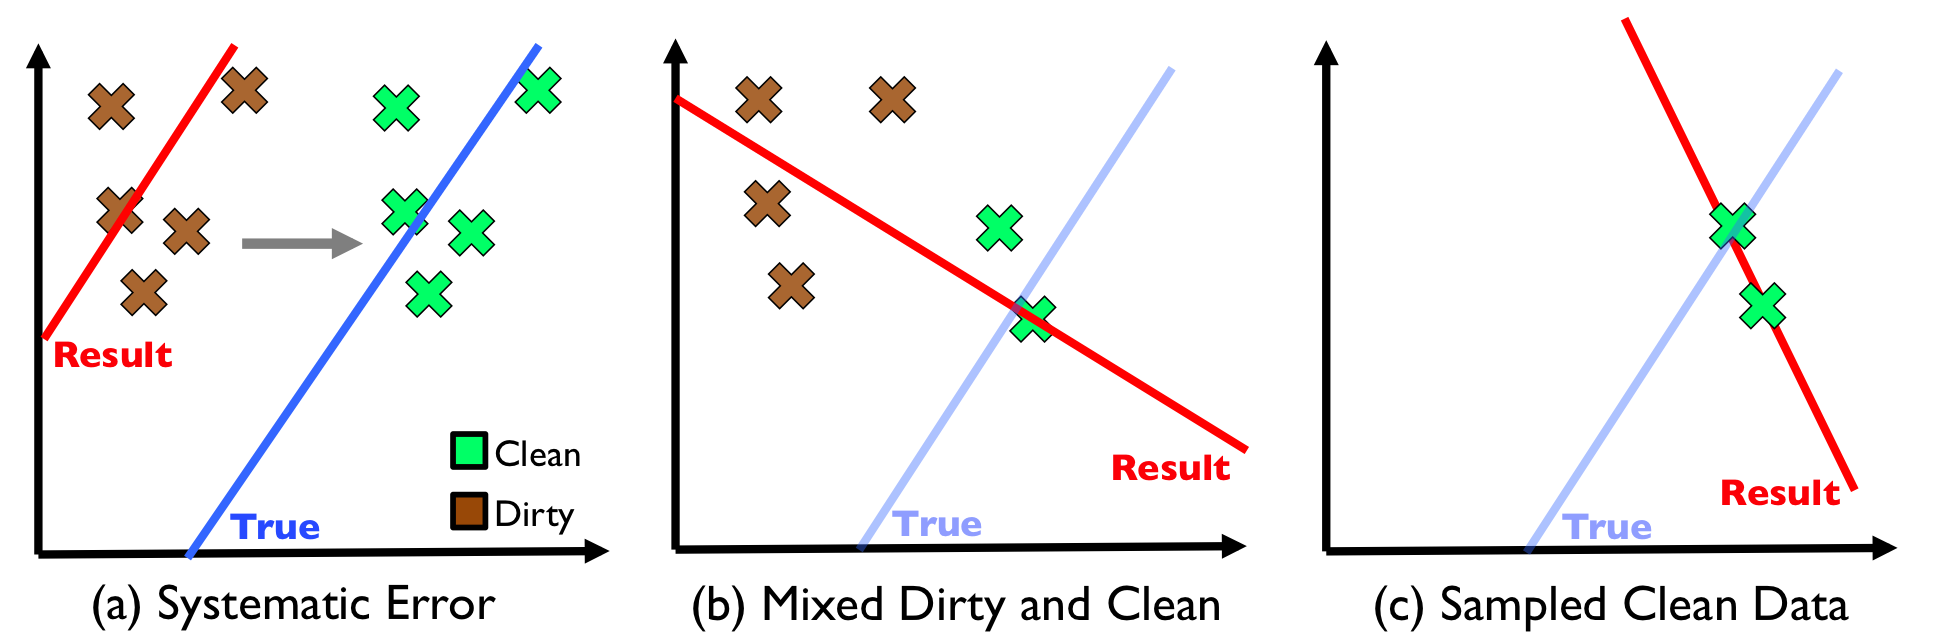
\includegraphics[width=0.6\columnwidth]{figs/update-arch.png}
 \caption{(a) Systematic corruption in one variable can lead to a shifted model. 
 (b) Mixed dirty and clean data results in a less accurate model than no cleaning.
(c) Small samples of only clean data can result in similarly inaccurate models. \label{update-arch1}}
\end{figure}

An alternative is to avoid the dirty data altogether instead of mixing the two populations.
Suppose $k$ records are randomly sampled from the dataset and cleaned.
The model is trained only on the cleaned sample of data.
This is similar to SampleClean \cite{wang1999sample}, which was proposed to approximate the results of aggregate queries by applying them to a clean sample of data.
However, high-dimensional models are highly sensitive to sample size.
Figure \ref{update-arch1}c illustrates that, even in two dimensions, models trained from small samples can be as incorrect as the mixing solution described before.

\subsection{ActiveClean}
In ActiveClean, we propose a new methodology to avoid Simpson's Paradox and the strong dependence on sample size.
Instead of mixing dirty and clean data, ActiveClean uses a model trained on the dirty data as an initialization, and then iteratively updates this model using samples of clean data.
The intuition is that this algorithm smoothly transitions the model from one population (the dirty data) to another (the clean data), leading to provable guarantees about intermediate results.

This work focuses on an initial class of well analyzed predictive analytics problems; ones that can be expressed as the minimization of convex loss functions.
Examples includes all generalized linear models (including linear and logistic regression), all variants of support vector machines, and in fact, means and medians are also special cases. 

Formally, for labeled training examples $\{(x_{i},y_{i})\}_{i=1}^{N}$, the problem is to find a vector of \emph{model parameters} $\theta$ by minimizing a loss function $\phi$ over all training examples:
\[
 \theta^{*}=\arg\min_{\theta}\sum_{i=1}^{N}\phi(x_{i},y_{i},\theta)
\]
Where $\phi$ is a convex function in $\theta$.
Typically, a \emph{regularization} term $r(\theta)$ is added to this problem.
$r(\theta)$ penalizes high or low values of feature weights in $\theta$ to avoid overfitting to noise in the training examples.
\[
 \theta^{*}=\arg\min_{\theta}\sum_{i=1}^{N}\phi(x_{i},y_{i},\theta) + r(\theta)
\]
Without loss of generality, we will include the regularization as part of the loss function i.e., $\phi(x_{i},y_{i},\theta)$ includes $r(\theta)$.

\begin{definition}[Convex Data Analytics]
A convex data analytics problem is specified by a set of features $X$, corresponding set of labels $Y$, and a parametrized loss function $\phi$ that is convex in its parameter $\theta$.
The result is a \textbf{model} $\theta$ that minimizes the sum of losses over all features and labels.
\end{definition}

\begin{figure}[t]
\centering
 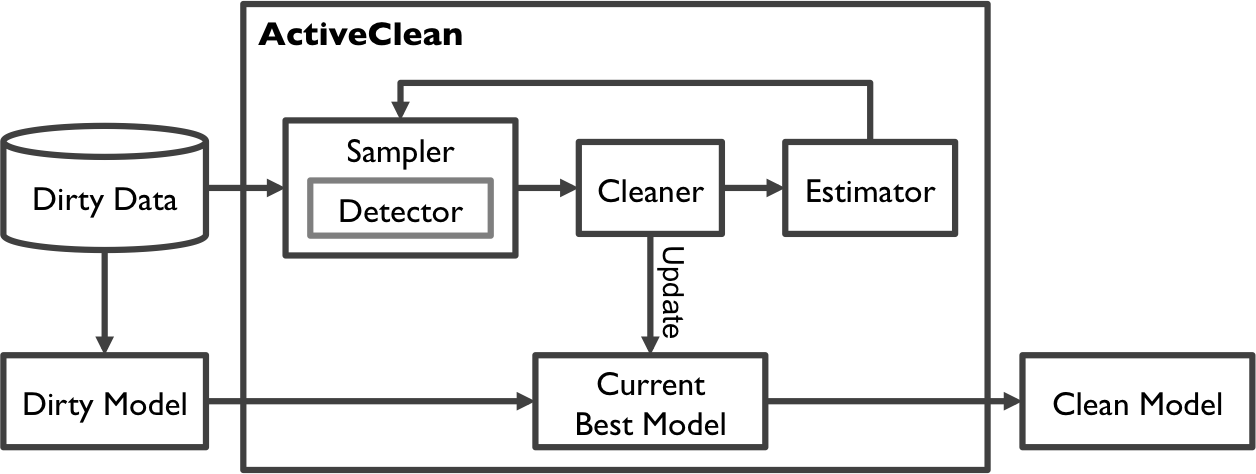
\includegraphics[width=0.5\columnwidth]{figs/arch2.png}
 \caption{ActiveClean is an architecture where data cleaning is integrated with model training in a framework with sampling, model update, and feedback through estimation. \label{sys-arch}}\vspace{-2em}
\end{figure}

\subsection{Framework and Architecture}
Rather than cleaning before model training, data cleaning can be directly integrated into the training process, so that ActiveClean can ensure provable guarantees such as convergence and error bounds.
In ActiveClean, data are cleaned in small random batches and the model is incrementally updated based on the results.
Similar to Active Learning, ActiveClean selects the most valuable records to clean with higher probability, however, it applies a number of optimizations that exploit the data cleaning setting such as avoiding data that is expected to be clean, estimating of the effect of data cleaning for a record, and batching together updates from already cleaned data.
This framework is optimized for problems that require expensive data cleaning.
Figure \ref{sys-arch} overviews the entire framework.

\noindent\textbf{Initialization: } There is a dirty relation $R$, a featurization $F(\cdot)$, a data cleaning technique $C(\cdot)$, and a dirty model $\theta^{(d)}$ trained on the featurized dirty relation.

\vspace{0.5em}

\noindent\textbf{Detector: } The first challenge in ActiveClean is dirty data detection. In this step, the detector select a candidate set of dirty records $R_{dirty} \subseteq R$. There are two techniques to do this: (1) an \emph{a priori} case, and (2) and an adaptive case. In the \emph{a priori} case, the detector knows which data is dirty in advance. In the adaptive case, the detector learns classifier based on previously cleaned data to detect corruption in uncleaned data.

\vspace{0.5em}

\noindent\textbf{Sampler: } The sampler draws a sample of records $S_{dirty} \subseteq R_{dirty}$. This is a non-uniform sample where each record $r$ has a sampling probability $p(r)$.
We derive the theoretical minimum variance sampling distribution, which is impossible to realize as it requires knowing the clean data in advance. Therefore, we use a first order first-order approximation of this distribution based on estimates of the clean data. 

\vspace{0.5em}

\noindent\textbf{Update: } This step updates the model $\theta^{(t)}$ based on the featurized (with featurization $F(\cdot)$) cleaned sample $F(S_{clean})$ resulting in $\theta^{(t+1)}$. The update procedure is a gradient descent step, and following from the convex model, this step gives bounded error for each iteration.

\vspace{0.5em}

\noindent\textbf{Estimator: } The estimator approximates the optimal distribution derived in the Sample step. Based on the change in the featurized data $F(S_{clean})$ and $F(S_{dirty})$, it directs the next iteration of sampling to select points that will have changes most valuable to the next model update.



